%% LyX 2.0.7 created this file.  For more info, see http://www.lyx.org/.
%% Do not edit unless you really know what you are doing.
\documentclass[a4paper,spanish]{scrreprt}
\usepackage{beraserif}
\usepackage{berasans}
\usepackage{beramono}
\usepackage[T1]{fontenc}
\usepackage[latin9]{inputenc}
\setcounter{tocdepth}{3}
\usepackage{color}
\usepackage{babel}
\addto\shorthandsspanish{\spanishdeactivate{~<>}}

\usepackage{graphicx}
\usepackage[authoryear]{natbib}
\usepackage[unicode=true,
 bookmarks=false,
 breaklinks=false,pdfborder={0 0 0},backref=false,colorlinks=true]
 {hyperref}
\hypersetup{
 urlcolor=webbrown,linkcolor=Blue,citecolor=webgreen,linktocpage=true,pageanchor=true,hypertexnames=false,naturalnames=true,plainpages=false}
\usepackage{breakurl}

\makeatletter

%%%%%%%%%%%%%%%%%%%%%%%%%%%%%% LyX specific LaTeX commands.
\special{papersize=\the\paperwidth,\the\paperheight}


%%%%%%%%%%%%%%%%%%%%%%%%%%%%%% Textclass specific LaTeX commands.
% use Latin Modern instead of Computer Modern sans serif
\renewcommand{\sfdefault}{lmss}

%%%%%%%%%%%%%%%%%%%%%%%%%%%%%% User specified LaTeX commands.
% book example for classicthesis.sty
 % KOMA-Script book
\usepackage{lipsum}
\usepackage[linedheaders,parts]{classicthesis}% ,manychapters
\usepackage[left=1in,right=0.7in,top=1in,bottom=1.5in]{geometry}

\makeatother

\begin{document}
\begin{titlepage}
\begin{addmargin}[0mm]{0.5in}  %%%%% symmetrical margins
%\usepackage[left=1.5in,right=1in,top=1in,bottom=1.5in]{geometry}
\large
\hfill

\vfill{}


\begin{center}
\begingroup \color{Maroon} \spacedallcaps{Integraci�n de clustering difuso y modelos deformables para la segmentaci�n de im�genes m�dicas} \endgroup\\
\bigskip{}
\spacedlowsmallcaps{Carmen Escudero Leoz y Manuel Corrales}
\par\end{center}

\begin{center}
\vfill{}

\par\end{center}

\begin{center}
\textbf{Directora }Mariana del Fresno\\
\textbf{Codirector }Jos� Ignacio Orlando
\par\end{center}

\begin{center}
\vfill{}

\par\end{center}

\begin{center}
\includegraphics[width=6cm]{\string"Logo UNICEN azul\string".eps}\\
 \medskip{}

\par\end{center}

\begin{center}
%Universidad Nacional del Centro de la Provincia de Buenos Aires Facultad de Ciencias Exactas
\par\end{center}

\medskip{}


\begin{center}
Trabajo final presentado para obtener el t�tulo de Ingeniero de Sistemas\\
%\myFaculty\\
%\myUni\\

\par\end{center}

\vfill{}


\end{addmargin} 
\end{titlepage} 


\cleardoublepage{}

\chapter{Introducción}
En los últimos años se ha experimentado un crecimiento notorio en lo que respecta a nuevas tecnologías aplicadas a la captura y al procesamiento de imágenes digitales. Estas herramientas han tenido un notable impacto en áreas de lo más diversas, siendo una de las más importantes la medicina. 

El surgimiento de nuevos procedimientos para el análisis y procesamiento de diversas modalidades de imágenes médicas tanto 2D como 3D ha permitido facilitar y mejorar la capacidad de los profesionales médicos para diagnosticar diferentes tipo de enfermedades o patologías. De igual manera, estas tecnologías han facilitado la exploración del interior del organismo humano con un grado de invasividad mucho menor al usual, dependiendo de la modalidad de imagen utilizada. En igual sentido, la vinculación estadística entre la información extraída a partir de las imágenes y distintas enfermedades ha contribuido al desarrollo de estudios científicos epidemiológicos merced a los cuales se ha dado lugar a nuevas investigaciones clínicas y nuevos tratamientos médicos.

La difusión de este tipo de tecnologías ha dado lugar al surgimiento de una de las áreas de estudio más importantes dentro del campo del Procesamiento de Imágenes y la Visión Computacional, conocida como Procesamiento de Imágenes Médicas, o Medical Imaging.

Una de las tareas más importantes dentro del área del Procesamiento de Imágenes
Médicas consiste en la identificación de regiones de interés (tales como órganos o lesiones), para su posterior caracterización y análisis \citep{pham2000current}. Este proceso es tradicionalmente conocido como segmentación, y constituye actualmente uno de los campos de investigación más explorados por parte de las ciencias de la computación. Dependiendo de la modalidad de imagen empleada y de los algoritmos desarrollados, diferentes resultados obtenidos han dado lugar a aplicaciones muy diversas, abarcando principalmente áreas tales
como la planificación de tratamientos médicos, la cirugía asistida por imágenes y la investigación en ciencia clínica, entre otras \citep{bankman2008handbook}.

\section{Descripción de la problemática}
Debido a que la segmentación de imágenes depende enormemente del tipo de imágenes a procesar y de la aplicación concreta en la que los resultados serán utilizados, se trata de un área en constante exploración y evolución, que converge hacia diversas soluciones dependiendo siempre de los factores anteriormente mencionados \cite{Bankman_2009}. Sin embargo, en el estado del arte es posible hallar diversas estrategias medianamente estandarizadas, tanto automáticas como interactivas, que permiten abordar este problema desde una perspectiva mayormente general, y que luego pueden ser especializadas a casos específicos. Estos enfoques en general pueden clasificarse en dos grandes grupos, supervisados y no supervisados. Los métodos supervisados hacen uso de datos de entrenamiento (sobre los que usuarios expertos han identificado las diferentes regiones que se desean segmentar) para adaptar un modelo (tradicionalmente, un clasificador) que sea capaz de diferenciarlas por sus propios medios. Los métodos no supervisados, por el contrario, no utilizan datos previamente etiquetados, si no que se adaptan a la solución por sus propios medios. Esto obliga a este tipo de enfoques a tener en cuenta la mayor cantidad de información que haya disponible dentro de las imágenes, a los efectos de mejorar su capacidad de discriminación.

Entre los métodos no supervisados de segmentación, el algoritmo de clustering conocido como Fuzzy C-Means es uno de los más utilizados. El mismo permite, a partir de diferentes descriptores extraídos  de la imagen (tales como indicadores de borde, intensidades, texturas, morfológicos, etc.), obtener automáticamente y sin intervención de ningún usuario experto C mapas difusos que detallan con cuánta probabilidad cada punto pertenece a C regiones de interés diferentes. Así, y dependiendo del valor mínimo de probabilidad tolerado, es posible posteriormente realizar una extracción binaria de cada una de las regiones, para su posterior cuantificación o análisis. Debido a que este tipo de algoritmos hace uso de un proceso iterativo que se basa en un análisis incremental de la distribución estadística de los valores de los descriptores, los resultados obtenidos dependen en gran medida de cuán buenos estos sean para diferenciar las estructuras a identificar. Para la segmentación de algunas estructuras de interés particulares tales como los tejidos principales del cerebro, la información relativa a la distribución espacial de los objetos en la imagen o a la proximidad entre píxeles o vóxeles ya identificados como pertenecientes a una determinada región permitiría mejorar sustancialmente los resultados obtenidos por un algoritmo como Fuzzy C-Means. Sin embargo, la integración de estas características no resulta sencilla, y en general requiere redefinir completamente el modelo iterativo estándar sobre el que el algoritmo se basa.

Otro método no supervisado utilizado comúnmente para la segmentación de imágenes médicas es Snakes, también conocido como Modelos Deformables o Superficies Activas. Este algoritmo se basa en la deformación de un contorno o membrana elástica a partir de información extraída de la imagen, y permite en general obtener representaciones suaves y con precisión sub-píxel o sub-vóxel de las estructuras a identificar. Una de sus mayores ventajas tiene que ver con las características intrínsecas del contorno deformable, dado que el mismo es una estructura conexa que crece y decrece sin perder su continuidad, e incorpora píxeles o vóxeles a la región conforme los mismos se asemejan a aquellos ya encerrados por la misma. Sin embargo, tradicionalmente estos métodos están basados únicamente en el estudio de las intensidades y los bordes en la imagen, y no permiten la incorporación de múltiples descriptores sin modificar de manera previa las definiciones de las fuerzas involucradas.

En este trabajo se propone la integración de ambos métodos de segmentación, Fuzzy C-Means y Snakes, en un único pipeline de procesamiento que permita, por un lado, la incorporación de la información provista por múltiples descriptores al esquema de fuerzas de las Snakes (mediante el uso de los mapas de pertenencia obtenidos por el método de clustering), y, por el otro, incorporar información relativa a la distribución de los píxeles en la estructura de interés (tomando ventaja de las características de conectividad de las membranas deformables del método de superficies activas).
\section{Organización del trabajo}
En este documento se describe en profundidad un método de segmentación que integra clustering difuso con superficies activas para la segmentación volumétrica de regiones de interés en imágenes médicas tridimensionales. El mismo fue evaluado para la tarea particular de detectar los principales tejidos que componen el cerebro (materia blanca y gris, y líquido cerebroespinal o cefalorraquídeo) a partir de imágenes de resonancia magnética 3D.

En el Capítulo \ref{chapter:estado_del_arte} se presenta un estudio del Estado del Arte de cada tema relevante. Particularmente en la sección \ref{section:procesamiento} se describen los fundamentos del procesamiento de imágenes médicas desde su captura hasta su procesamiento para la utilización en diagnóstico y toma de decisiones. En la sección \ref{section:algoritmos} se aborda una descripción de los algoritmos de segmentación describiendo brevemente cada uno.

El Capítulo \ref{chapter:metodos} es uno de los principales capítulos de este trabajo ya que se presenta el método propuesto de segmentación. Se inicia con una descripción general del esquema en la sección \ref{section:descripcion_general} continuando con una explicación de la segmentación de Fuzzy C-Means siendo el primer algoritmo involucrado. En la Sección \ref{section:extraccion_de_mallas} se describe brevemente el proceso de extracción de mallas que es el paso previo y cuya salida es utilizada en la última etapa del método. Esta última etapa es descrita en la Sección \ref{section:modelos_deformables} donde se presenta inicialmente Modelos Deformables, se continua con el Modelo continuo de Contornos Activos y luego la discretización del mismo. Por último en la Sección \ref{section:estudio_de_sensibilidad} se incluye un estudio de sensibilidad del algoritmo presentado en el capítulo con el fin de obtener parámetros adecuados para la ejecución de los experimentos.

Para finalizar, se presentan los resultados obtenidos en el Capítulo \ref{chap:resultados} detallando los datos utilizados para las pruebas, las métricas obtenidas y una evaluación cuantitativa y cualitativa del esquema propuesto.

Como corolario en el Capítulo \ref{chap:conclusiones} se incluyen las conclusiones a las que se arribó al finalizar este trabajo así como también potenciales trabajos futuros.


\chapter{Reporte 1: Fuzzy C-Means}


\section{Introducci�n}

Como se explic� anteriormente, la etapa inicial de nuestro enfoque
de segmentaci�n est� basada en Fuzzy C-Means. Fuzzy C-Means es un
algoritmo de clustering no supervisado que permite obtener segmentaciones
difusas agrupando elementos similares en clusters. Un cluster es un
conjunto de elementos que son afines entre s�. Una de las principales
desventajas de los algoritmos de clustering tradicionales radica en
que los mismos asumen que cada elemento pertenece inequ�vocamente
a un cluster, ignorando si existe o no alguna similaridad con los
dem�s miembros de otros clusters (full1982fuzzy). Una manera de modelar
esta similaridad fue introducida por Zadeh en 1965 \citet{zadeh1965fuzzy},
y consiste en representar la semejanza de los puntos que se desean
clusterizar con una funci�n cuyos valores est�n entre cero y uno.
Basado en esta propuesta, y a diferencia de K-Means, en donde cada
elemento pertenece o no a un cluster de manera determinante, en Fuzzy
C-Means cada elemento posee una probabilidad de pertenencia a cada
uno de los clusters. Este agrupamiento se obtiene minimizando iterativamente
una funci�n de costo que depende de la similaridad de los elementos
de un cluster respecto al centroide del mismo. El centroide es el
vector caracter�stico de un cl�ster, obtenido como el promedio de
los vectores de caracter�sticas de los puntos que pertenecen al cluster.
A cada cl�ster le corresponde un �nico centroide, que var�a conforme
se incorporan o quitan puntos del mismo. Fuzzy C-Means requiere como
entrada un vector de caracter�sticas por cada uno de los puntos que
se desean clusterizar, y el n�mero de clusters en los que se quiere
dividir la imagen. El algoritmo asigna a cada voxel a una categor�a
con una cierta probabilidad de pertenencia. M�s formalmente, sea $X=(x_{1},x_{2},...,x_{n})$
una imagen de $n$ voxeles a ser particionados en $C$ regiones, en
donde cada $x_{i}$ representa el vector de caracter�sticas del $i$-�simo
v�xel. El algoritmo asigna cada v�xel a una clase a trav�s de la minimizaci�n
iterativa de una funci�n de costo, definida como: 

\[
formulaaca
\]


donde $u_{ij}$ representa la pertenencia de un voxel $x_{j}$ al
cluster $i$, $v_{i}$ es el centroide del cluster $i$, $\left|\right|$
es la distancia eucl�dea entre los voxels y m es una constante. Esta
constante controla el nivel de difusi�n de la clusterizaci�n resultante
\citet{chuang2006fuzzy}. La funci�n de costo tiene por objetivo asignar
probabilidades altas de pertenencia de un v�xel $j$ a un cluster
$i$ si su vector caracter�stico asociado $x_{j}$ es similar al centroide
$v_{j}$. Esta similitud entre vectores es cuantificada midiendo la
distancia eucl�dea entre ambos en el espacio de caracter�sticas: si
el vector de caracter�sticas es muy dis�mil respecto al centroide
del cluster de estudio, la distancia eucl�dea entre ambos ser� alta;
si los vectores son similares, la distancia ser� menor. El resultado
del proceso de segmentaci�n es una matriz de pertenencias y una lista
de centroides de cada una de las regiones. En las siguientes secciones
se abordar�n algunos detalles particulares del algoritmo, evaluados
sobre diferentes tipos de im�genes. En la Secci�n X.X se presenta
un estudio de sensibilidad realizado sobre fantomas artificiales con
y sin ruido, y con y sin efecto bias. En la Secci�n X.X describimos
un estudio similar realizado sobre im�genes de MRI cerebrales. 


\section{Estudio de sensibilidad sobre fantomas artificiales}

\begin{figure}
\begin{centering}
\includegraphics{images/mitad_mitad_250x250}
\par\end{centering}

\caption{Imagen artificial con clusters abiertos}
\end{figure}


\begin{figure}
\begin{centering}
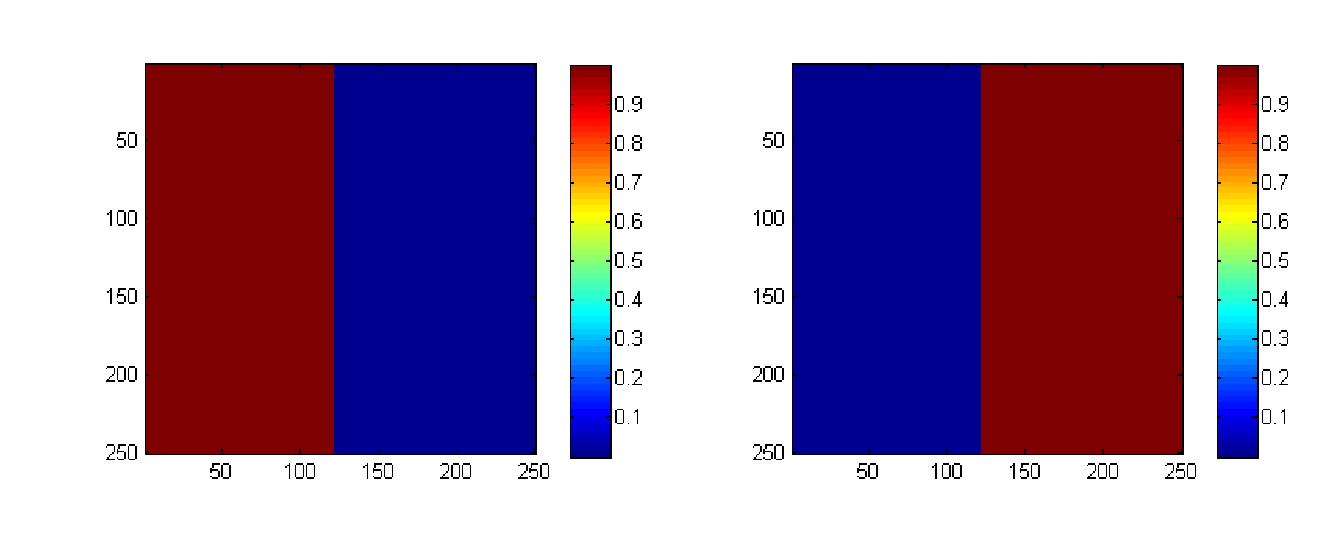
\includegraphics[scale=0.75]{images/mitad_mitad_clusters_sin_coordenadas_random}
\par\end{centering}

\caption{Clusterizacion con centroides aleatorios, sin coordenadas espaciales}
\end{figure}


\begin{figure}
\begin{centering}
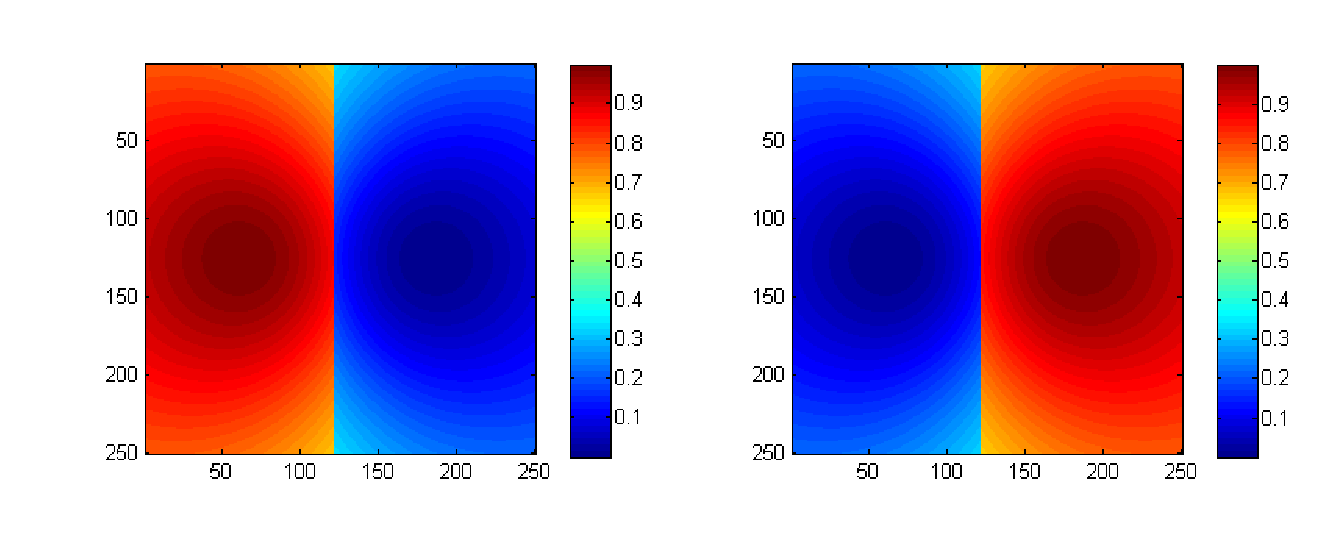
\includegraphics[scale=0.75]{images/mitad_mitad_clusters_con_coordenadas_random}
\par\end{centering}

\caption{Clusterizacion con centroides aleatorios y coordenadas espaciales}


\end{figure}


\begin{figure}
\begin{centering}
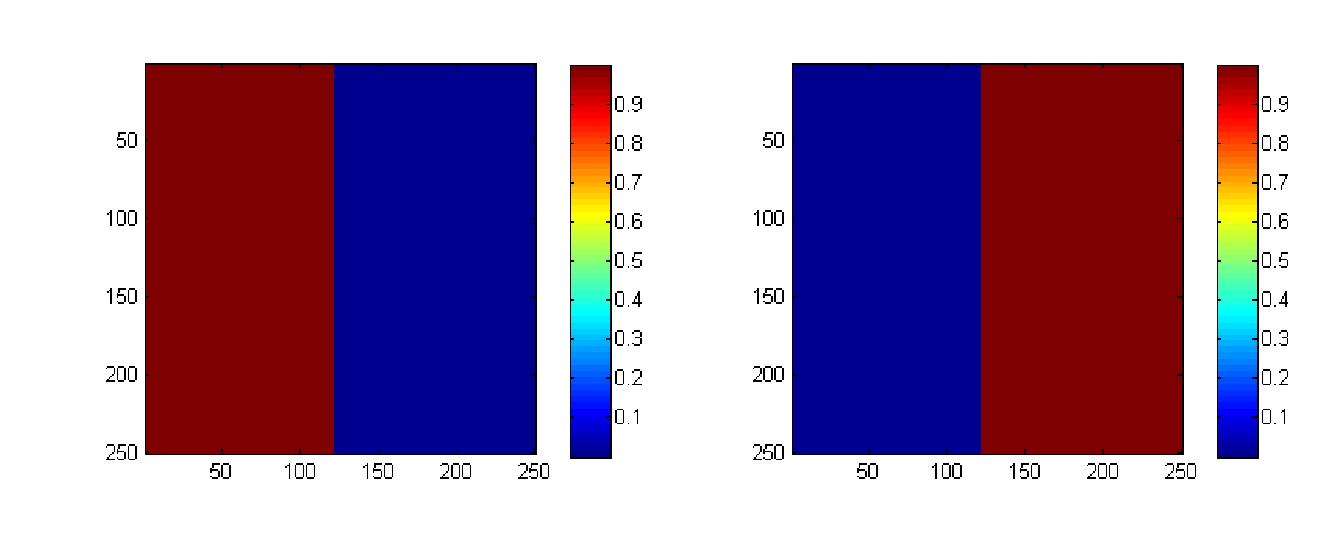
\includegraphics[scale=0.75]{images/mitad_mitad_clusters_sin_coordenadas_random}
\par\end{centering}

\caption{Clusterizacion con centroides iniciales seleccionados a mano sin coordenadas
espaciales}


\end{figure}


\begin{figure}
\begin{centering}
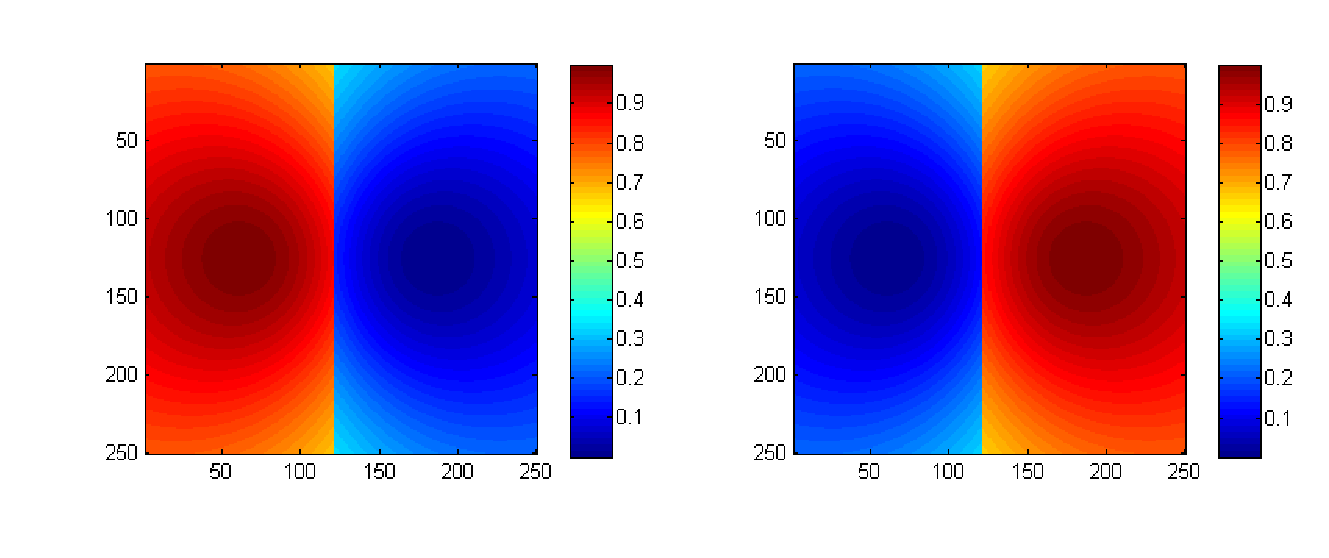
\includegraphics[scale=0.75]{images/mitad_mitad_clusters_con_coordenadas_centroide_manual}
\par\end{centering}

\caption{Clusterizacion con centroides iniciales seleccionados a mano y coordenadas
espaciales}


\end{figure}


\begin{figure}
\begin{centering}
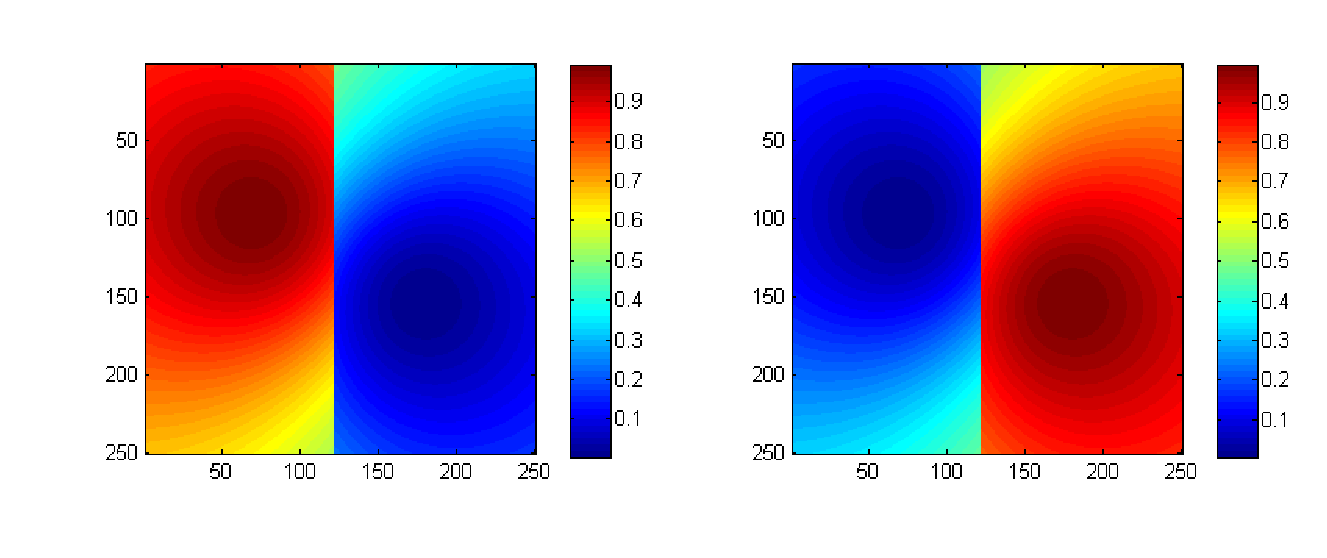
\includegraphics[scale=0.75]{images/mitad_mitad_clusters_con_coordenadas_centroide_manual_1iteracion}
\par\end{centering}

\caption{Clusterizacion con centroides iniciales seleccionados a mano, coordenadas
espaciales con una sola iteracion}


\end{figure}


\begin{center}
\begin{figure}
\begin{centering}
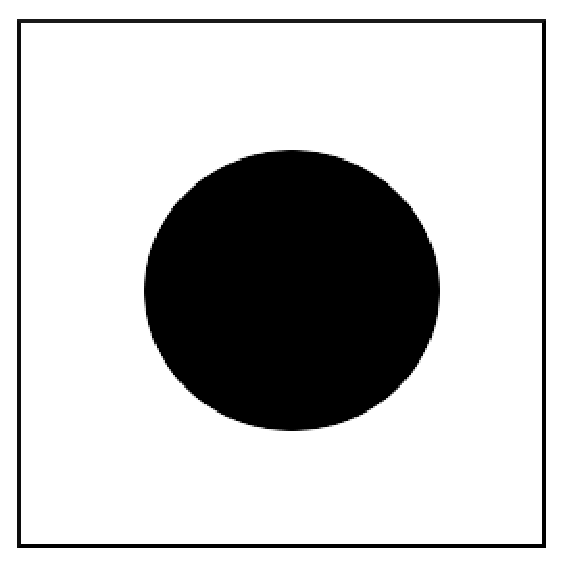
\includegraphics{images/circulo_250x250}
\par\end{centering}

\centering{}\caption{Imagen artificial zona cerrada}
\end{figure}

\par\end{center}




\cleardoublepage{}

\bibliographystyle{plainnat}
\phantomsection\addcontentsline{toc}{chapter}{\bibname}\bibliography{Tesis}

\end{document}
